\chapter{Spanning Tree Protocol: Part
2}\label{spanning-tree-protocol-part-2}

\section{STP States}\label{stp-states}

\begin{figure}
\centering
\pandocbounded{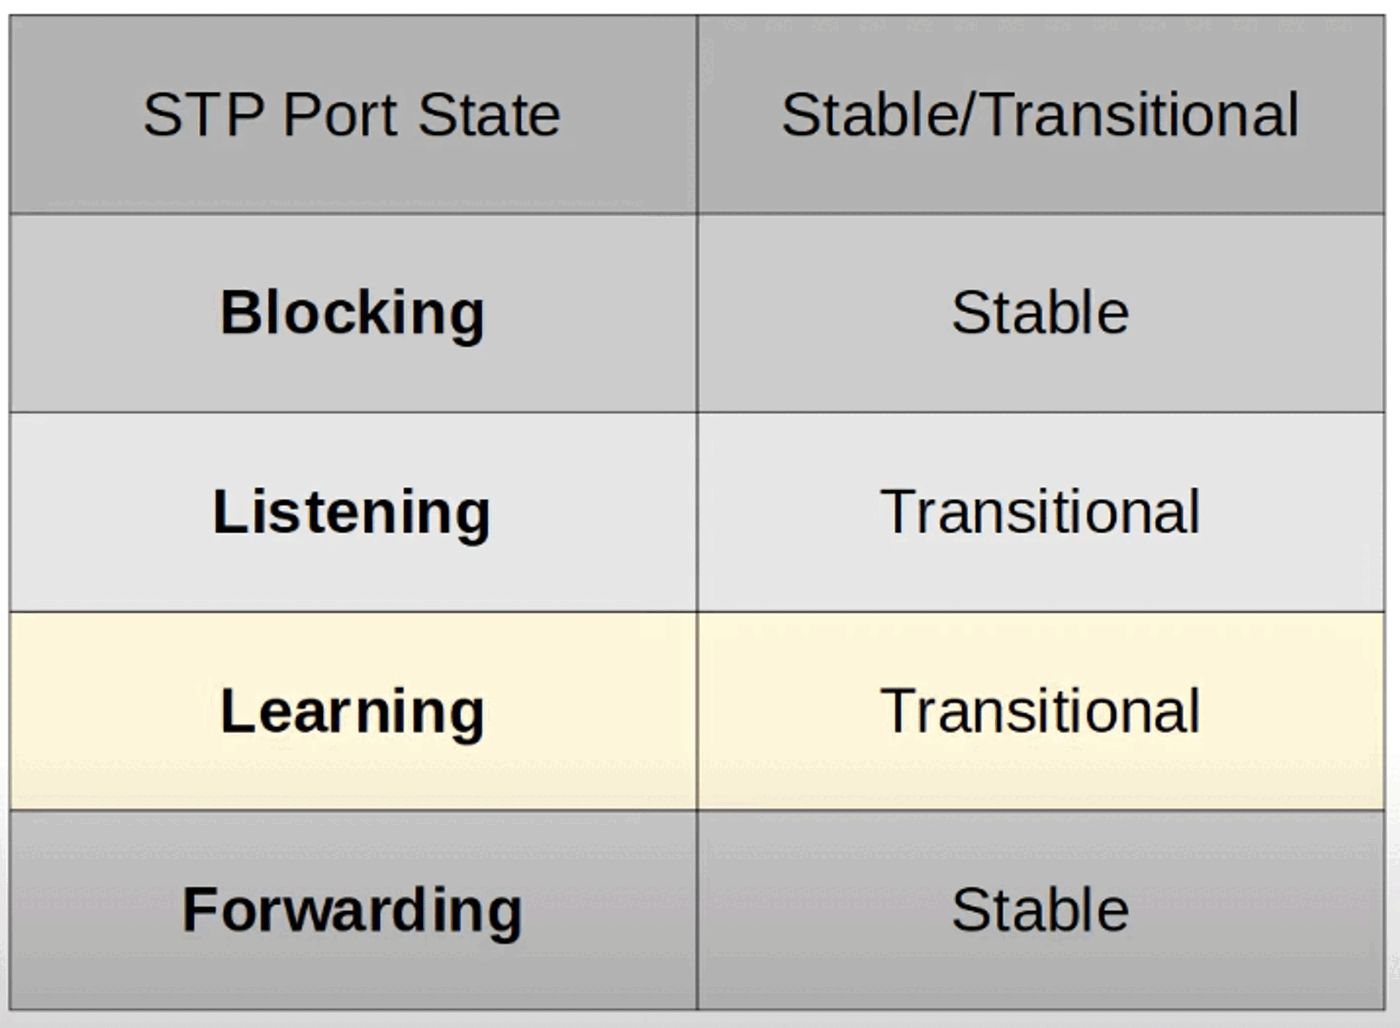
\includegraphics[keepaspectratio,alt={image}]{images/22-spanning-tree-protocol-part2/img-001.png}}
\end{figure}

\begin{itemize}
\tightlist
\item
  ROOT / DESIGNATED PORTS remain STABLE in a FORWARDING state
\item
  NON-DESIGNATED PORTS remain STABLE in a BLOCKING state
\item
  LISTENING and LEARNING are TRANSITIONAL states which are passed
  through when an interface is activated, or when a BLOCKING PORT must
  transition to a FORWARDING state due to a change in network topology.
\end{itemize}

\textbf{1) BLOCKING / STABLE}

\begin{itemize}
\tightlist
\item
  NON-DESIGNATED PORTS are in a BLOCKING state
\item
  Interfaces in a BLOCKING state are effectively disabled to prevent
  loops
\item
  Interfaces in a BLOCKING state do NOT Send/Receive regular network
  traffic
\item
  Interfaces in a BLOCKING state do NOT forward STP BPDUs
\item
  Interfaces in a BLOCKING state do NOT learn MAC ADDRESSES
\end{itemize}

\textbf{2) LISTENING / TRANSITIONAL}

\begin{itemize}
\tightlist
\item
  After the BLOCKING state, interfaces with the DESIGNATED or ROOT role
  enter the LISTENING state
\item
  ONLY DESIGNATED or ROOT PORTS enter the LISTENING state
  (NON-DESIGNATED PORTS are ALWAYS BLOCKING)
\item
  The LISTENING state is 15 seconds long by Default. This is determined
  by the FORWARD DELAY TIMER
\item
  Interfaces in a LISTENING state do NOT Send / Receive regular network
  traffic
\item
  Interfaces in a LISTENING state ONLY Forward/Receive STP BPDUs
\item
  Interfaces in a LISTENING state does NOT learn MAC ADDRESSES from
  regular traffic that arrives on the interface
\end{itemize}

\textbf{3) LEARNING / TRANSITIONAL}

\begin{itemize}
\tightlist
\item
  After the LISTENING state, a DESIGNATED or ROOT port will enter the
  LEARNING state
\item
  The LEARNING state is 15 seconds long by Default. This is determined
  by the FORWARD DELAY TIMER (same one used for both LISTENING and
  LEARNING states)
\item
  Interfaces in a LEARNING state do NOT Send / Receive regular network
  traffic
\item
  Interfaces in a LEARNING state ONLY Sends/Receives STP BPDUs
\item
  Interfaces in a LEARNING state \textbf{learns} MAC ADDRESSES from
  regular traffic that arrives on the interface
\end{itemize}

\begin{enumerate}
\def\labelenumi{\arabic{enumi})}
\setcounter{enumi}{3}
\tightlist
\item
  FORWARDING / STABLE
\end{enumerate}

\begin{itemize}
\tightlist
\item
  ROOT and DESIGNATED PORTS are in a FORWARDING state
\item
  A PORT in the FORWARDING state operate as NORMAL
\item
  A PORT in the FORWARDING state Sends/Receives regular network traffic
\item
  A PORT in the FORWARDING state Sends/Receives STP BPDUs
\item
  A PORT in the FORWARDING state \textbf{learns} MAC ADDRESSES
\end{itemize}

\section{Summary}\label{summary}

\begin{figure}
\centering
\pandocbounded{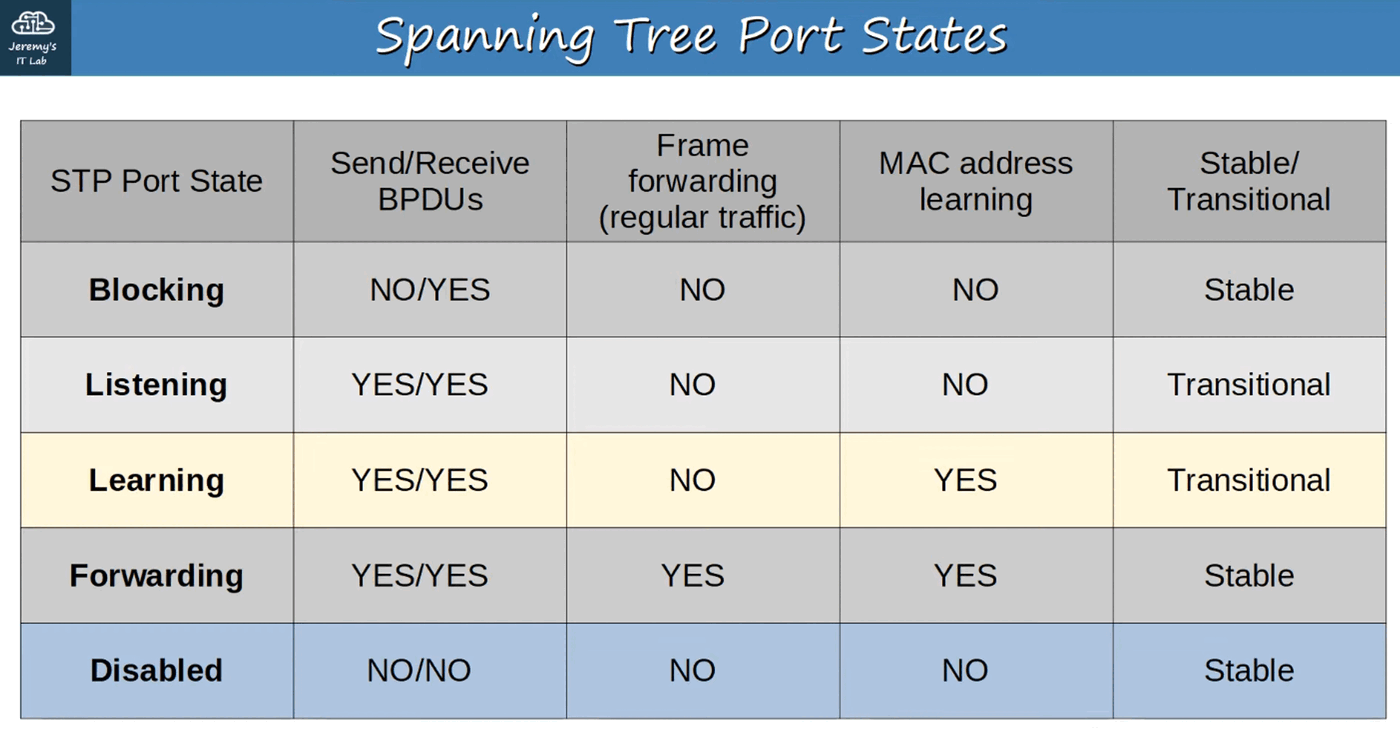
\includegraphics[keepaspectratio,alt={image}]{images/22-spanning-tree-protocol-part2/img-002.png}}
\end{figure}

\section{STP Timers}\label{stp-timers}

\begin{figure}
\centering
\pandocbounded{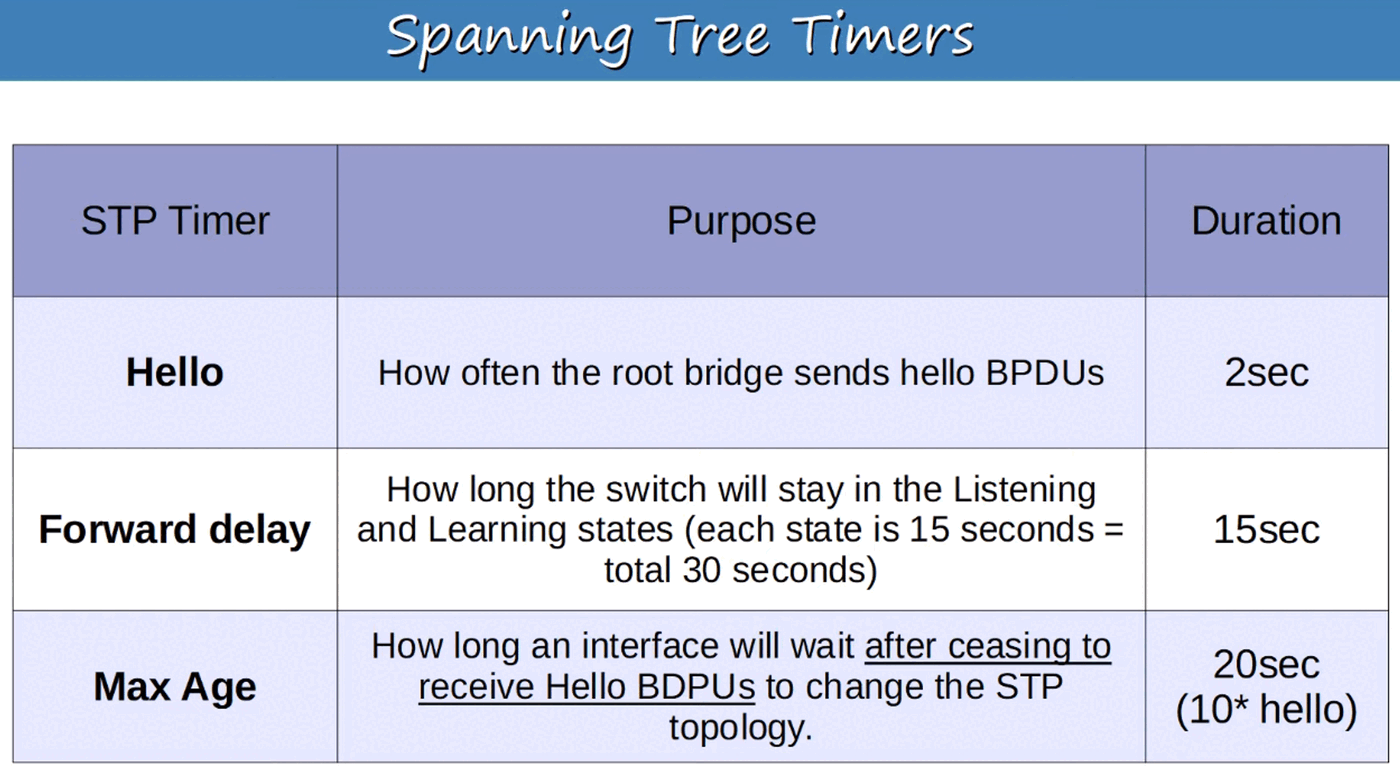
\includegraphics[keepaspectratio,alt={image}]{images/22-spanning-tree-protocol-part2/img-003.png}}
\end{figure}

SWITCHES do NOT forward the BPDUs out of their ROOT PORTS and
NON-DESIGNATED PORTS - ONLY their DESIGNATED PORTS !!!

\section{Max Age Timer}\label{max-age-timer}

\begin{itemize}
\tightlist
\item
  If another BPDU is received BEFORE MAX AGE TIMER counts down to 0, the
  TIME will RESET to 20 Seconds and no changes will occur.
\item
  If another BPDU is not received, the MAX AGE TIMER counts down to 0
  and the SWITCH will re-evaluate it's STP choices, including ROOT
  BRIDGE, LOCAL ROOT, DESIGNATED, and NON-DESIGNATED PORTS.
\item
  If a NON-DESIGNATED PORT is selected to become a DESIGNATED or ROOT
  PORT, it will transition from the BLOCKING state to the LISTENING
  state (15 Seconds), LEARNING state (15 Seconds), and then finally the
  FORWARDING state.

  \begin{itemize}
  \tightlist
  \item
    So\ldots{} it can take 50 Seconds for a BLOCKING interface to
    transition to FORWARDING! (MAX AGE TIMER + (LISTENING + LEARNING 15
    Second timers))
  \end{itemize}
\item
  These TIMERS and TRANSITIONAL STATES are to make sure that LOOPS are
  not accidentally created by an INTERFACE moving to FORWARDING STATE
  too soon
\end{itemize}

HOWEVER \ldots{}

A FORWARDING interface can move DIRECTLY to a BLOCKING state (there is
no worry about creating a loop)

A BLOCKING interface can NOT move DIRECTLY to a FORWARDING state. It
MUST go through the LISTENING and LEARNING states first!

\section{STP BPDU (Bridge Protocol Data
Unit)}\label{stp-bpdu-bridge-protocol-data-unit}

Ethernet Header of a BPDU

\begin{figure}
\centering
\pandocbounded{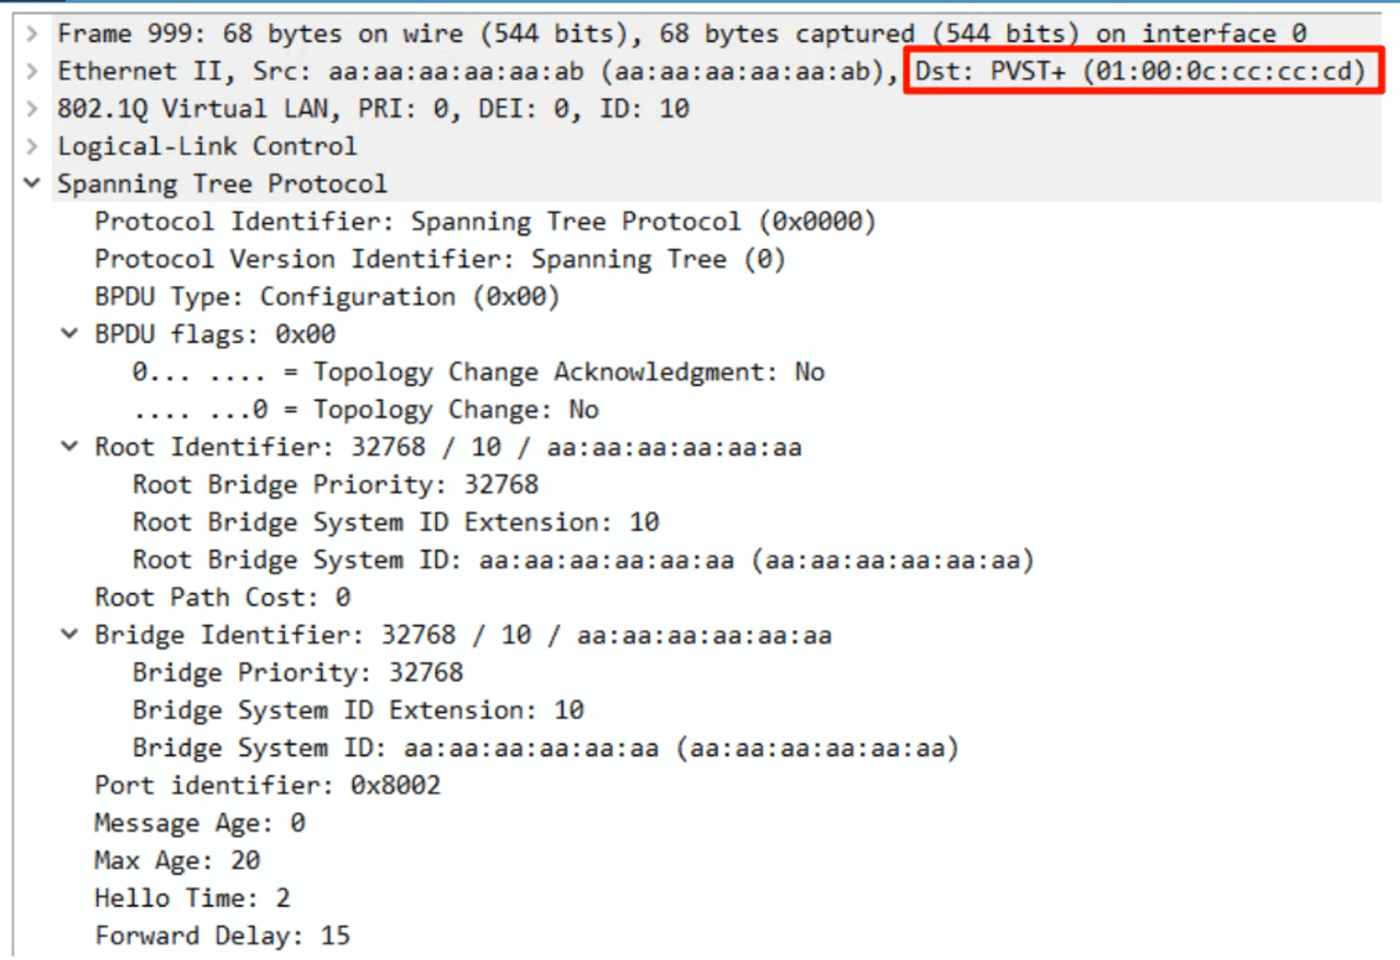
\includegraphics[keepaspectratio,alt={image}]{images/22-spanning-tree-protocol-part2/img-004.png}}
\end{figure}

PVST+ uses the MAC ADDRESS :

01 : 00 : 0c : cc : cc : cd

PVST = ONLY ISL Trunk Encapsulation

PVST+ = Supports 802.1Q

Regular STP (not Cisco's PVST+) uses the MAC ADDRESS :

01 : 80 : c2 : 00 : 00 : 00

The STP TIMERS on the ROOT BRIDGE determine ALL STP TIMERS for the
entire network!

\section{STP Optional Features (STP
Toolkit)}\label{stp-optional-features-stp-toolkit}

\section{Portfast}\label{portfast}

\begin{itemize}
\tightlist
\item
  Can be Enabled on INTERFACES which are connected to END HOSTS
\end{itemize}

PORTFAST allows a PORT to move immediately to the FORWARDING state,
bypassing LISTENING and LEARNING

\begin{itemize}
\tightlist
\item
  If used, it MUST be ENABLED only on PORTS connected to END HOSTS
\item
  If ENABLED on a PORT connected to another SWITCH, it could cause a
  LAYER 2 LOOP
\end{itemize}

\begin{figure}
\centering
\pandocbounded{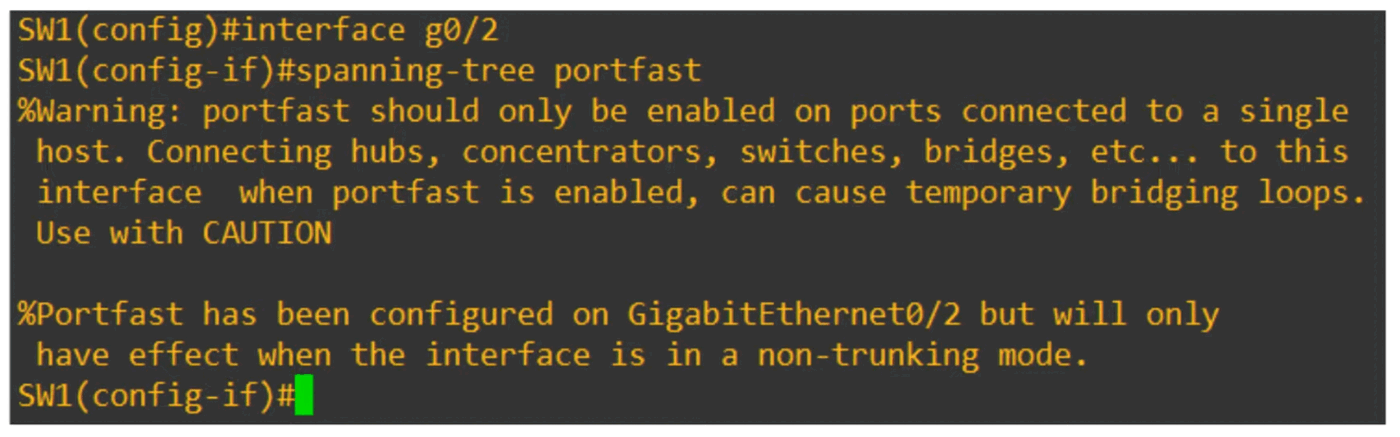
\includegraphics[keepaspectratio,alt={image}]{images/22-spanning-tree-protocol-part2/img-005.png}}
\end{figure}

You can also ENABLE PORTFAST with the following command:

SW1(config)\# spanning-tree portfast default

This ENABLES PORTFAST on ALL ACCESS PORTS (not TRUNK PORTS)

\section{BPDU Guard}\label{bpdu-guard}

\begin{itemize}
\tightlist
\item
  If an INTERFACE with BPDU GUARD ENABLED receives a BPDU from another
  SWITCH, the INTERFACE will be SHUT DOWN to prevent loops from forming.
\end{itemize}

\begin{figure}
\centering
\pandocbounded{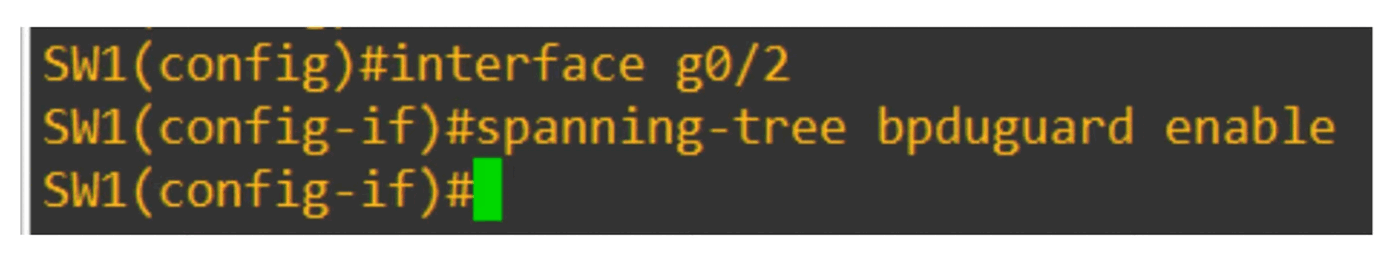
\includegraphics[keepaspectratio,alt={image}]{images/22-spanning-tree-protocol-part2/img-006.png}}
\end{figure}

You can also ENABLE BPDU GUARD with the following command:

SW1(config)\# spanning-tree portfast bpduguard default

This ENABLES BPDU GUARD on all PORTFAST-enabled INTERFACES

\section{Root Guard / Loop Guard}\label{root-guard-loop-guard}

\begin{figure}
\centering
\pandocbounded{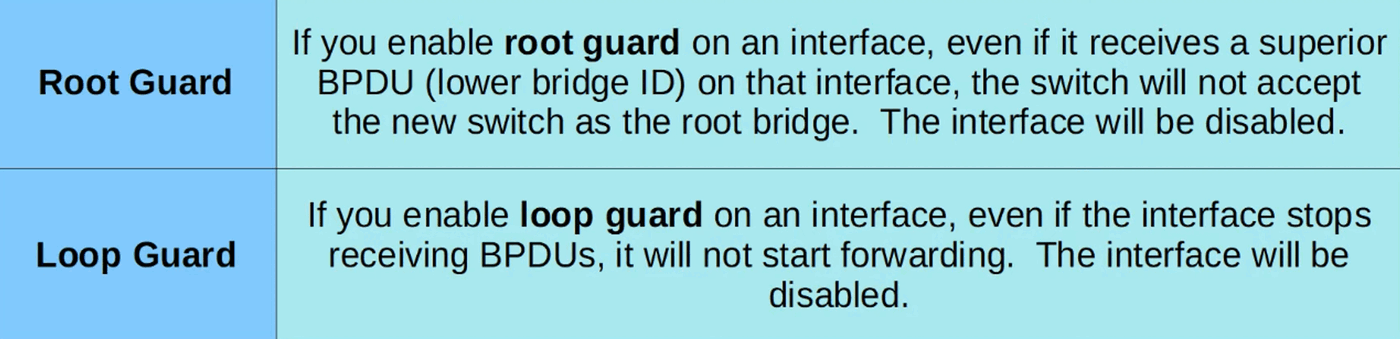
\includegraphics[keepaspectratio,alt={image}]{images/22-spanning-tree-protocol-part2/img-007.png}}
\end{figure}

You probably do NOT have to know these STP optional features (or others
such as UplinkFast, Backbone Fast, etcetera) for the CCNA.

BUT\ldots{}

Make sure you know PORTFAST and BPDU GUARD.

\section{STP Configuration}\label{stp-configuration}

Command to CONFIGURE Spanning-Tree mode on a SWITCH

\begin{figure}
\centering
\pandocbounded{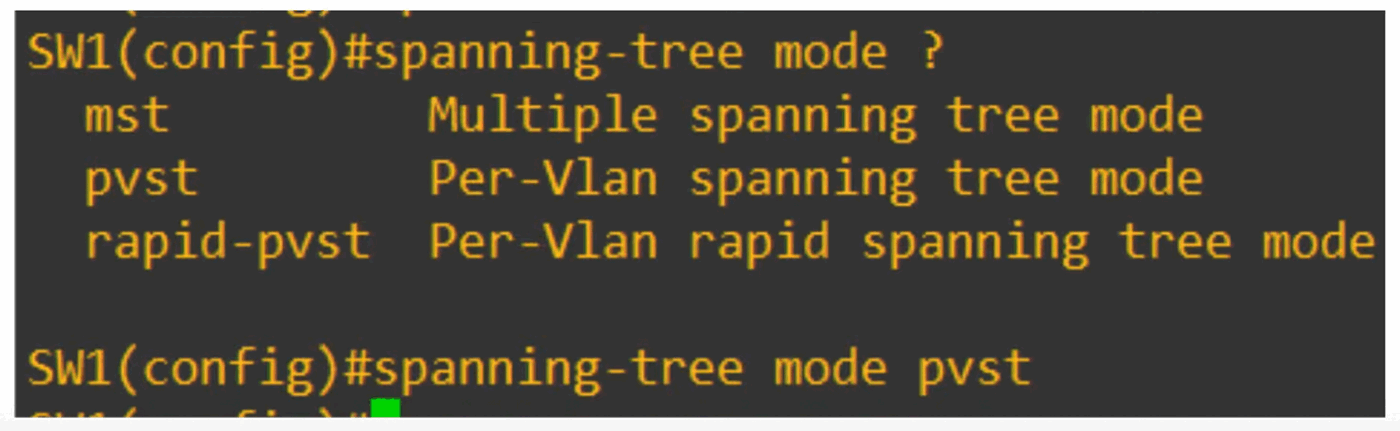
\includegraphics[keepaspectratio,alt={image}]{images/22-spanning-tree-protocol-part2/img-008.png}}
\end{figure}

Modern Cisco SWITCHES run \textbf{rapid-pvst}, by default

\section{Configure the Primary Root
Bridge}\label{configure-the-primary-root-bridge}

Command to CONFIGURE Spanning-Tree PRIMARY ROOT BRIDGE on a SWITCH

\begin{figure}
\centering
\pandocbounded{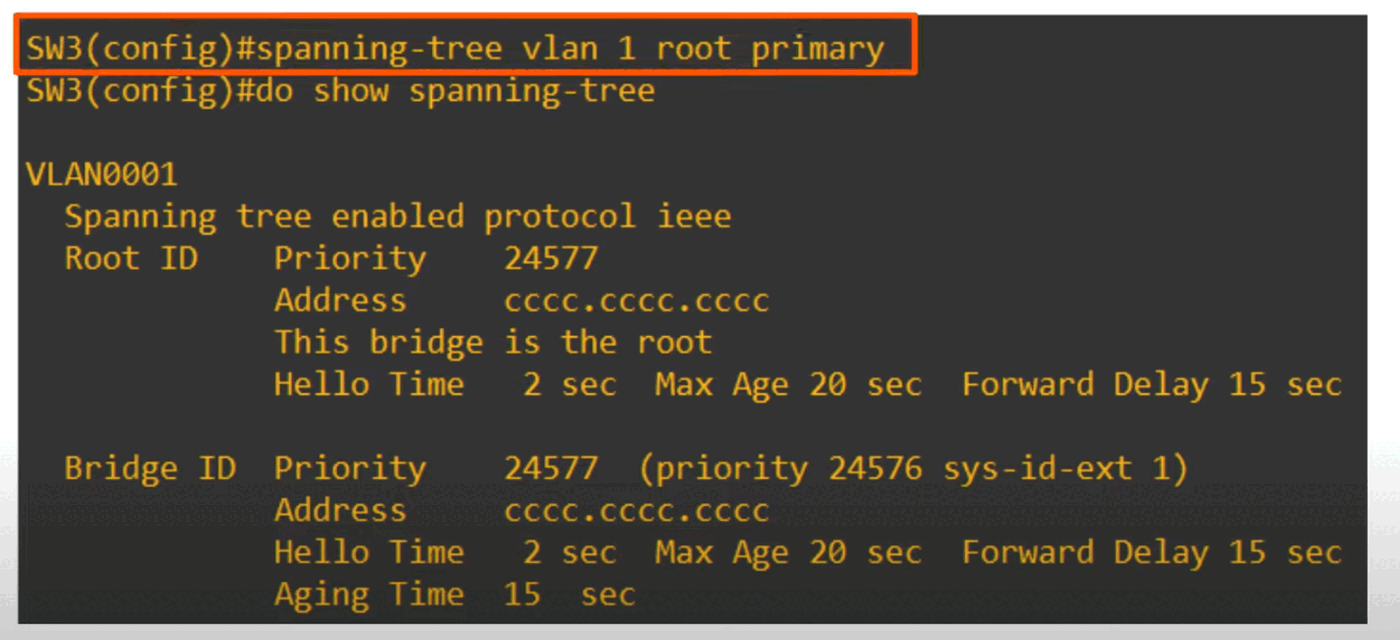
\includegraphics[keepaspectratio,alt={image}]{images/22-spanning-tree-protocol-part2/img-009.png}}
\end{figure}

Confirm with ``(do) show spanning-tree''

Can see in the above example, SW3 has become the ``root''

\begin{itemize}
\tightlist
\item
  The ``spanning-tree vlan \textless vlan-number\textgreater{} root
  primary'' command sets the STP PRIORITY to 24576. If another SWITCH
  already has a priority number lower than 24576, it sets this SWITCH's
  priority to 4096 LESS THAN the other SWITCH's Priority (remember STP
  PART 1 lecture)
\end{itemize}

SECONDARY ROOT BRIGE (backup ROOT BRIDGE)

Command to CONFIGURE Spanning-Tree SECONDARY ROOT BRIDGE on a SWITCH

\begin{figure}
\centering
\pandocbounded{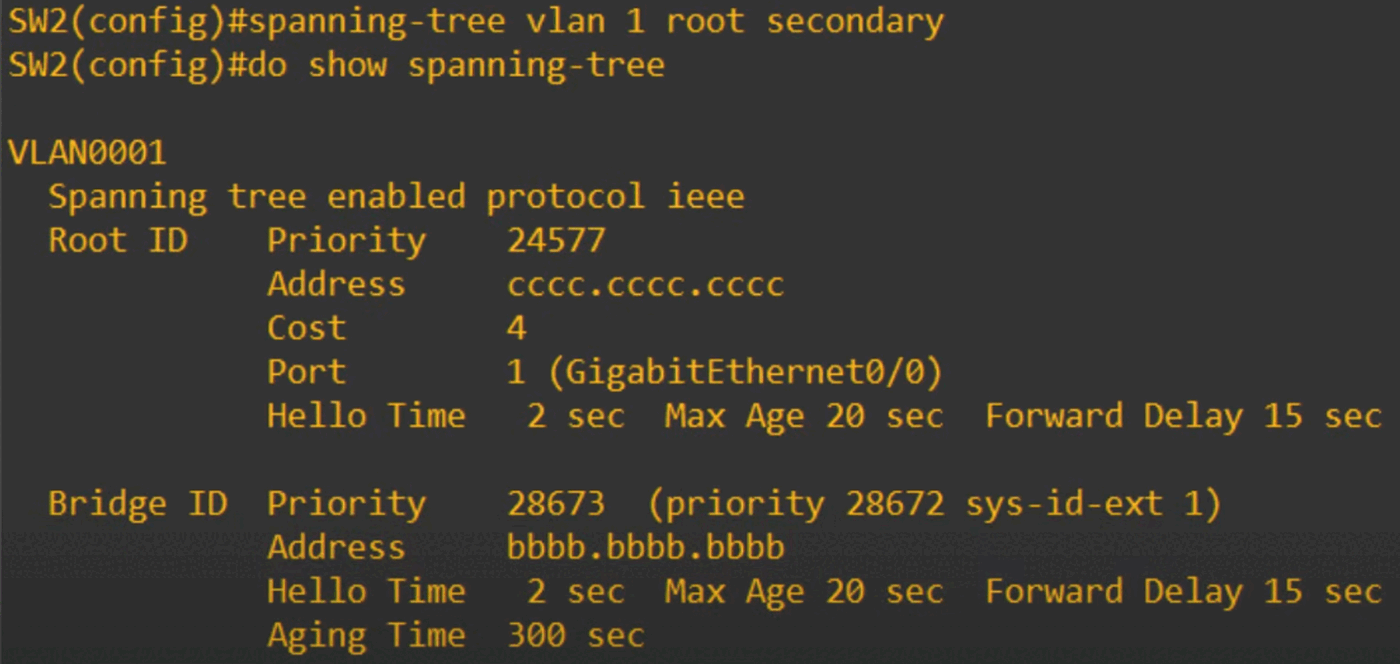
\includegraphics[keepaspectratio,alt={image}]{images/22-spanning-tree-protocol-part2/img-010.png}}
\end{figure}

\begin{itemize}
\tightlist
\item
  The ``spanning-tree vlan \textless vlan-number\textgreater{} root
  secondary'' command sets the STP PRIORITY to 28672 (exactly 4096
  higher than 24576).
\end{itemize}

VLAN 1 TOPOLOGY running PVST+

\begin{figure}
\centering
\pandocbounded{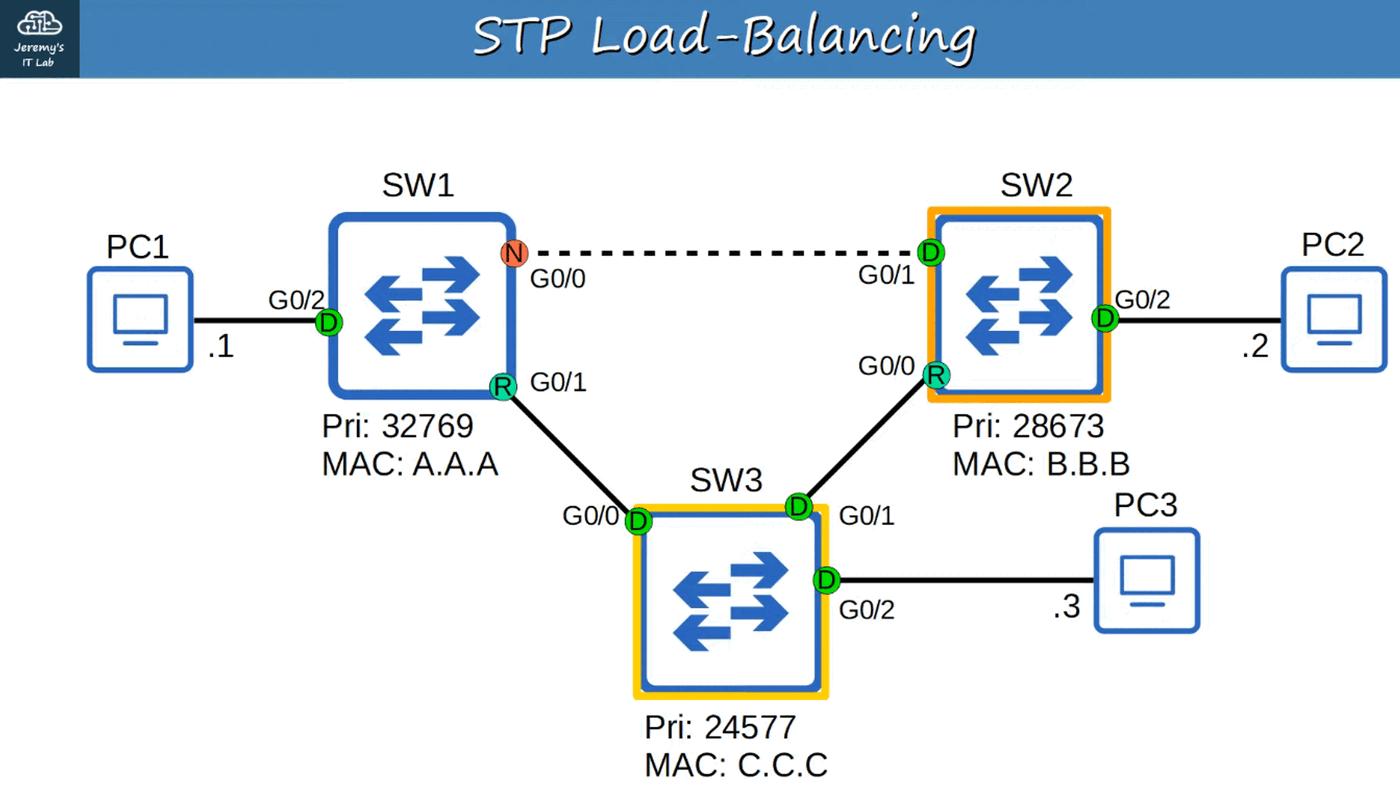
\includegraphics[keepaspectratio,alt={image}]{images/22-spanning-tree-protocol-part2/img-011.png}}
\end{figure}

SW1 WAS the PRIMARY ROOT BRIDGE but :

\begin{itemize}
\tightlist
\item
  We have configured SW3 to be the PRIMARY
\item
  We have configured SW2 to be the SECONDARY
\end{itemize}

The TOPOLOGY for VLAN 2, however, won't be the same. It will be the OLD
Topology.

\begin{figure}
\centering
\pandocbounded{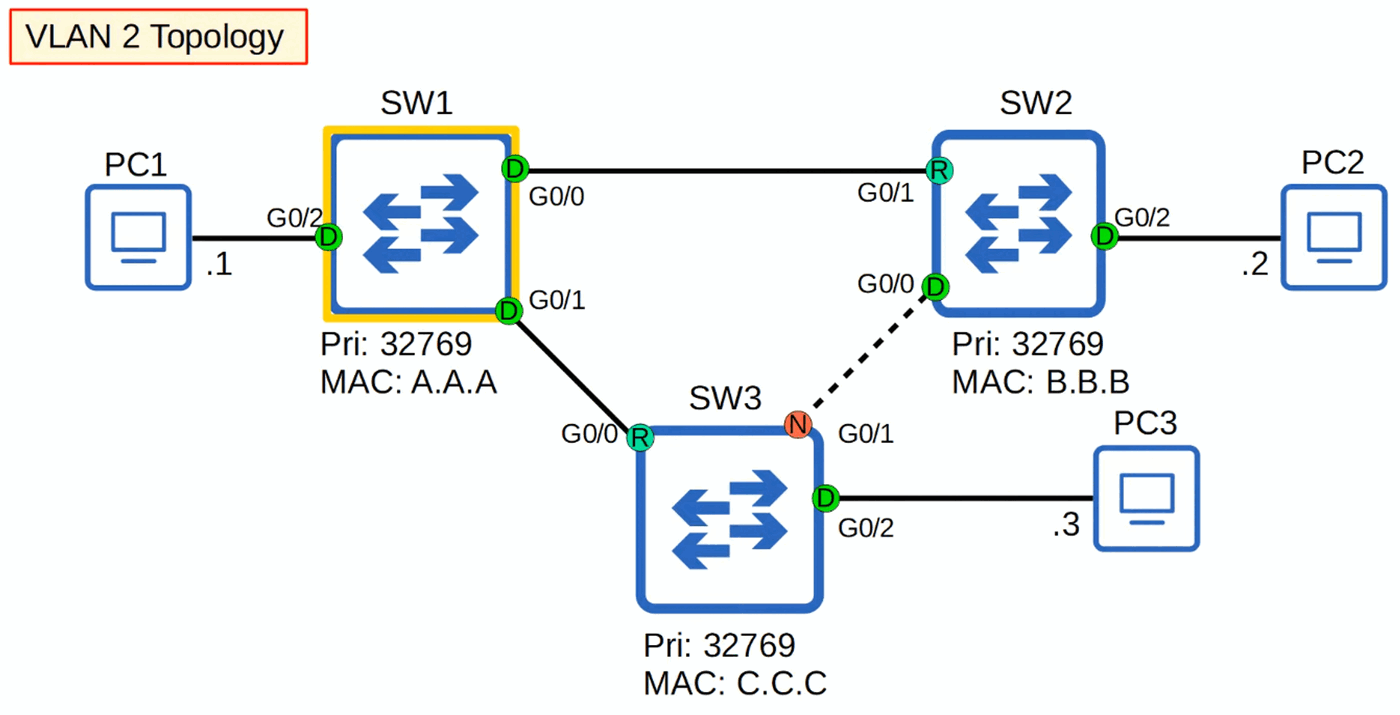
\includegraphics[keepaspectratio,alt={image}]{images/22-spanning-tree-protocol-part2/img-012.png}}
\end{figure}

WHY? Because we made changes ONLY to the TOPOLOGY found in VLAN 1 (see
the commands we used)

\section{Configure STP Port Settings}\label{configure-stp-port-settings}

\begin{figure}
\centering
\pandocbounded{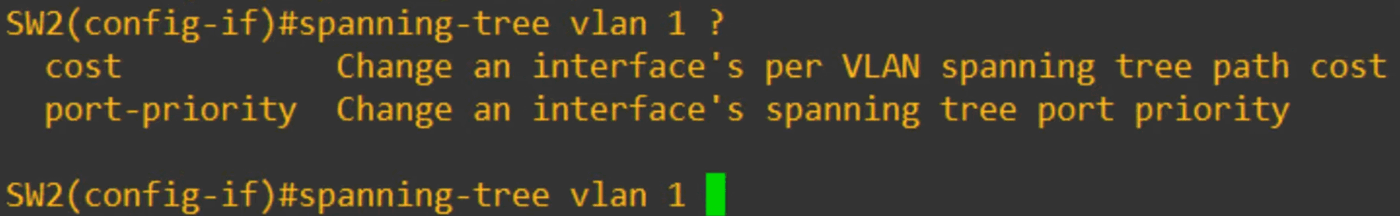
\includegraphics[keepaspectratio,alt={image}]{images/22-spanning-tree-protocol-part2/img-013.png}}
\end{figure}

``cost'' = ``ROOT COST''

``port-priority'' = ``PORT PRIORITY''
